% !TeX program = xelatex
% !TeX encoding = UTF-8
\documentclass[UTF8]{standalone}
\usepackage{amsmath,fourier,ctex,tikz}
\begin{document}
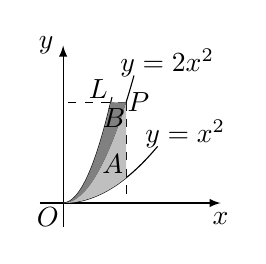
\begin{tikzpicture}[domain=-0.3:3]
	\draw[-latex] (-0.3,0) node[left=-3pt,below=-2pt] {$O$} -- (2,0) node[below] {$x$};
	\draw[-latex] (0,-0.3) -- (0,2) node[left] {$y$};
	\draw[domain=0:1.2] plot (\x,{0.5*\x^2}) node[right=10pt,above=-4pt] {$y = x^{2}$};
	\draw[domain=0:0.9] plot (\x,{2*\x^2}) node[right=12pt,above=-4pt] {$y = 2x^{2}$};
	\draw[domain=0:0.62] plot (\x,{3.5*\x^2}) node[above=3pt,left=-2pt] {$L$};
	\draw[dashed] (0.8,2*0.8^2) -- (0,2*0.8^2);
	\draw[dashed] (0.8,2*0.8^2) -- (0.8,0);
	\fill [fill = lightgray] [domain = 0:0.8,smooth] plot (\x, {pow(\x,2)/2}) -- (0.8,2*0.8^2) [domain = 0.8:0, smooth] -- plot (\x, {2*pow(\x,2)}) -- cycle;
	\fill [fill = gray] [domain = 0:0.8,smooth] plot (\x, {2*pow(\x,2)}) -- (0.60474,2*0.8^2) [domain = 0.60474:0, smooth] -- plot (\x, {3.5*pow(\x,2)}) -- cycle;
	\node at (0.645,2*0.8^2-0.2) {$B$};
	\node at (0.63,0.5) {$A$};
	\node[right=-3pt] at (0.8,2*0.8^2) {$P$};
\end{tikzpicture}
\end{document}